%\documentclass[11pt,dvipdfm]{article}
\documentclass[11pt]{article} %The above line must be used for your camera-ready submission, which requires %a latex -> DVI -> PDF compilation pipeline. As a workaround while you are writing your paper, you could %comment it out and use this line instead, which is compatible with pdflatex.


\usepackage{authblk}
\usepackage{deauthor,times,hyperref} 
%\usepackage[utf8]{inputenc}
\usepackage{underscore}
\usepackage{graphicx}
\usepackage{soul}
\usepackage{url}
\def\UrlBreaks{\do\/\do-}
\newtheorem{requirement}{Req.}

\begin{document}

\title{Towards Privacy by Design for Data with \MakeUppercase{strm} privacy}

\author{
  Bart van Deenen\\
  \small{strmprivacy.io}
  \and
  Pim Nauts\\
  \small{strmprivacy.io}
  \and
  Robin Trietsch\\
  \small{strmprivacy.io}
  \and
  Bart Voorn\\
  \small{strmprivacy.io \&}\\
  \small{University of Amsterdam}
}
\maketitle



%%%%%%%%%%%%%%%%%%%%%%%%%%%%%%%%%%%%%%%%%%%%%%%%%%%%%%%%%%%%%%%%%%%%%%%%%%%%%%%
%                                Abstract
%%%%%%%%%%%%%%%%%%%%%%%%%%%%%%%%%%%%%%%%%%%%%%%%%%%%%%%%%%%%%%%%%%%%%%%%%%%%%%%

\begin{abstract}
Both societal and regulatory pressure (GDPR) increasingly challenge organizations and engineering teams to balance privacy and innovation. Striking this balance can be costly in terms of effort, data utility and computation costs. Moreover, current approaches in scalable data systems often treat privacy as an access problem, which is at odds with important legal and design principles. A plethora of privacy preserving- and enhancing- technologies are available, yet their adoption in production data systems still faces challenges. In particular, their focus is often on narrow use cases such as external data sharing, on mostly existing data sets, rendering them unusable in real-time data architectures. In this paper we argue engineering teams should ``shift left`` with their data privacy efforts, to the point of data collection. We show how privacy challenges in production architectures can be addressed without compromising speed, data quality or privacy. We provide a detailed yet practical explanation of an architectural set-up that allows users to launch privacy streams in seconds. 
\end{abstract}

%%%%%%%%%%%%%%%%%%%%%%%%%%%%%%%%%%%%%%%%%%%%%%%%%%%%%%%%%%%%%%%%%%%%%%%%%%%%%%%
%                                Introduction
%%%%%%%%%%%%%%%%%%%%%%%%%%%%%%%%%%%%%%%%%%%%%%%%%%%%%%%%%%%%%%%%%%%%%%%%%%%%%%%

\section{Introduction}

If the industrial revolution ran on fossil fuel, modern-day organizations run on data. From governments to hospitals, manufacturing to digital marketplaces: data systems are everywhere and have quickly become a core asset and capability to deploy for any modern organization in order to innovate. With``data`` driving both considerable value creation and grounded concern about the impact to private individuals, legislators developed and implemented new regulations like the General Data Protection Regulation (GDPR) \cite{GDPR} in the European Union to foster innovation without foregoing individual rights to privacy \cite{bridge2018} . 

But even in \textit{data-native} organizations, precisely this ``balancing'' of privacy and data driven innovation is not an easy task for data engineers, privacy officers and data governance experts alike. While the first foundational work on \textit{Privacy by Design} from Ann Cavoukian dates back to the 90s \cite{cavoukian1997}, building modern, scalable data systems around privacy principles is still a nascent field due to a lack of (technical) standards and a prolonging gap between the policy perspective and operational reality of data systems \cite{abiteboul2019transparency}. This gap leads to a very real ``Cost of Privacy`` to organizations beyond just legal costs \cite{bhajaria2022data}. Structuring privacy operations in organizations, at scale, requires time and effort. Increased coordination across departments, unclarity around requirements, longer development cycles, additional staffing for e.g. RTBF requests \cite{korenhof2015timing} and ``privacy paralysis``\footnote{the observation that taking a next step with application development is delayed or even refrained from due to privacy concerns} all mean organizations incur additional- and opportunity costs. For example, a structured approach to privacy is often lacking, and the GDPR requirements around data collection and user opt-ins lead to reverse-engineering the legal ground and related purpose for collecting and processing data, with engineering teams often pulled into lengthy legal discussions on purpose. Moreover, requirements like strong anonymization pose a practical challenge to data utility and -usability for (data) engineering teams. 

Despite this apparent \textit{Cost of Privacy}, available solutions are still limited. We see the gap between the policy perspective and real-world systems is most apparent in the way privacy is embedded in many data architectures. Often, privacy is treated as an access problem on data that is already collected, stored and used\footnote{e.g. the way many modern data warehouses deal with privacy is through role-based access}, not as a first principle of systems design (often without traceability to the collection ground and collection purpose). While this is convenient as it requires limited re-architecting of existing systems, we believe this is an "early efficiency win [that causes] late stage headaches" \cite{bhajaria2022data}. Moreover, it is at odds with (if not in violation of) legislative directions. This often leads to (i) organizations accepting an increased risk profile or (ii) refraining from engaging in new use cases (and so innovation) altogether. All in, the current approach to dealing with privacy often poses another real cost and risk to organizations, both financial and in reputation. 

\subsection{Privacy Enhancing Technologies}
One of the domains where these challenges are being (partly) addressed, is in Privacy Enhancing or Privacy Preserving Technologies (PET's) \cite{Polonetsky2021review}. PET's allow data practitioners to transform sensitive data into usable input for consumption or support detecting sensitive data \cite{bhajaria2022data}, limiting risk of unsolicited data consumption. Yet, they have important shortcomings in the practical sense: they often center around external data sharing as the dominant use case, are computationally heavy, best suited to aggregate data operations only and/or rely on "complete" data sets. This makes them better suited to use cases where data is already collected and stored. Hence, PET's provide a solution for a limited set of use cases and can still lead to non-compliance with privacy regulations if data was not properly collected or bounded to data purpose \cite{bhajaria2022data}.

\subsection{Towards Privacy by Design for data}
To bridge the gap from the realities of privacy professionals and data (system) engineers to available technologies, we propose an architecture to encode privacy in data that helps to structure privacy efforts, and a system to implement this at lower real-world costs. Both the architecture and system come from a set of clear principles, derived from legal and privacy by design requirements:

\subsubsection{Requirements}
\begin{itemize}
  \item \textbf{\textit{Explicit contracting}} - define both data shape (the schema) and privacy implications as metadata (including key legislative concepts such as collection ground) in \underline{data contracts} that describe each datapoint. 
    \item \textbf{\textit{Enforce transformation}} - define %SSCFIX%\ul{privacy levels}
    inside the contracts, set per-field privacy transformations, such as de-identification or anonymization, for sensitive (PII\footnote{Personally Identifiable Information, such as a name or email}) data fields, so that data collection and processing are tightly coupled. 
  \item \textbf{\textit{Shift left}} - Enforce these data contracts \underline{at ingestion}, so data is (i) always bound to purpose and (ii) welded to the original collection ground.
  \item \textbf{\textit{Retain utility}} - transform data in such a way that the trade-off between privacy and utility is limited or even removed. 
  \item \textbf{\textit{Dedicated distribution}} - provide a dedicated interface for every specific collection ground through \underline{privacy streams}, so that applications and/or downstream users are guaranteed to only receive (i) necessary and (ii) properly transformed data.
  \item \textbf{\textit{Interoperable}} - the system should naturally complement existing architectures and accommodate \underline{easy integration and deployment}
   (aligned with industry standards). 
  \item \textbf{\textit{Cheap and Fast}} - extend interoperability by aiming to add minimal additional latency to existing systems and limit computational cost of operations.  
\end{itemize}

In effect, a solution should allow data teams to build with confidence, cut costly coordination time, and enable them to quickly deploy a contemporary (streaming) data infrastructure with a focus on high quality data at low effort at lower legal and reputation risks. 


%%%%%%%%%%%%%%%%%%%%%%%%%%%%%%%%%%%%%%%%%%%%%%%%%%%%%%%%%%%%%%%%%%%%%%%%%%%%%%%
%                                Challenges
%%%%%%%%%%%%%%%%%%%%%%%%%%%%%%%%%%%%%%%%%%%%%%%%%%%%%%%%%%%%%%%%%%%%%%%%%%%%%%%
\section{Limiting the Cost of Privacy: privacy, utility and design challenges}
In this section we identify the challenges that surround building scalable data systems from privacy forward, and the design principles that should shape them. We will approach these as drafting the list of requirements for building these \textit{Privacy by Design} data systems. 

\subsection{Privacy challenges}
\subsubsection{Key requirements from GDPR}
While often viewed as a complex legislation, the core of what GDPR seeks to achieve is straight forward: protection of individuals' private data. A few key concepts set the boundaries for responsible (and lawful) data behavior, such as accountability (you are accountable for the data you control), and data subject rights (what an individual can require from a controller). We will use these as a treasure map in hunting for requirements. 

\textbf{Data minimization and consent}
Of key interest to our challenge are the governing principles on how to collect and use data: data minimization and consent obligations. Simply put, they state one should not collect more data than necessary for a purpose, and can only collect data under \textit{either} explicit consent for that purpose or a justified cause\footnote{Consent, purpose and legal ground are used interchangeably}, like legitimate interest or contract fulfillment (e.g. an e-commerce marketplace simply needs your home address to deliver your order). 

In practice, these legal grounds are oftentimes liberally interpreted. Historical data -- i.e. data that has been collected in the past and stored in e.g. a data warehouse -- is often persisted without storing the purpose under which it was acquired. This is clearly problematic in the privacy sense: it is (nearly) impossible to determine the purpose of a data point after the data collection took place.

It becomes even more interesting once we acknowledge the dynamic nature of consent. For example, how do we handle changing preferences of end-users, and how is consent linked to data over time? By collecting purpose up-front, and ensuring that this purpose stays with the data, two problems are handled instantly: purpose limitation and consent \cite{soria2016big}. This yields the first challenge we should take into account:

\begin{requirement}
\textit{\textbf{We should encode how a data point was obtained and for what purpose}}
\end{requirement}

\textbf{Purpose limitation}
As data in practice is often collected once and then up- and recycled often, there is another key principle to take into account: purpose limitation. In the official text, GDPR article 5 section 1(b) \cite{GDPR}, we see the following:

\begin{quote}
    \textit{Personal data shall be collected for specified, explicit and legitimate purposes and not further processed in a manner that is incompatible with those purposes; further processing for archiving purposes in the public interest, scientific or historical research purposes or statistical purposes shall, in accordance with Article 89(1), not be considered to be incompatible with the initial purposes (‘purpose limitation’)}.
\end{quote}

This is directly at odds with the common practice of hoarding data into a warehouse. If the purpose of data collection is not clear, the legal ground cannot be determined and consent cannot legally be obtained \cite{soria2016big}. While the legalese and exact wording of what purposes can be considered legal is far outside of the scope of many data engineering professionals, this is a clear area of interest for designing systems around privacy: data usage without determining if it is legal to use for a certain purpose is already violating this very principle. In practice we see this judgement is often made by a data consumer team without (sufficient) knowledge of Personal Data regulations. This paves the way to our second requirement: 

\begin{requirement}
\textit{\textbf{Data consumers should only receive data they are entitled to, given the consent of the data-owner, for the specific purpose of the data consumer \footnote{processor in GDPR parlance}}}
\end{requirement}

So e.g. while a data-team building a recommender system has a vested interest in knowing what a user does, they do not need to know who the user is - and so could do with any random value representing the user as long as its consistent over time for that specific person or user account (provide consent or legal ground is present!). 

\subsubsection{Privacy by Design, the principles}
Our next source of system requirements are the original Privacy by Design principles laid out by Ann Cavoukian in her capacity as the Information and Privacy Commissioner of Ontario \cite{cavoukian1997}. 

The first principles\footnote{1. Proactive not Reactive; Preventative not Remedial, 2. Privacy as the Default Setting, 3. Privacy Embedded into Design} revolve around timing - when privacy comes into play in both designing systems and the flow of data. Clearly, it is only private by \textit{design} if "characterized by proactive rather than reactive measures, [anticipating and preventing] privacy invasive events before they happen". Moreover, the "maximum degree of privacy" is in warranting the protection of personal data in "any given" data system (aligning with our first requirement: encode privacy into data). This suggests a profound shift of the point at which privacy becomes part of the data flow:
\begin{requirement}
\textit{\textbf{Privacy should be embedded right where data is collected.}}
\end{requirement}

More recent views on best practices like Bhajaria's (2022) \cite{bhajaria2022data} also suggest that both classifying and tagging data before it hits data pipelines (i.e. at ingest) mitigates privacy risks more optimally.  

\subsection{Data utility}
\subsubsection{Bringing structure to data improves data quality}
Even before privacy comes into play, many data practitioners will recognize the challenge of data quality in and of itself. In organizations with lots of operational legacy systems (which does not imply they are "old"!), it is common to see the creative re-use of fields/columns in a data set. Dealing with confusing field names, undocumented changes in lineage and empty fields are common practice in the real world \cite{barhamgi2022special}. Moreover, data consumers generally have \emph{no direct control} on what is accepted as valid data, and will often have to resort to heuristics to determine what to do with a certain data field. 

\newpage Think of this as \textit{data debt} or negative interest building inside data flows. Adding and enforcing more structure in data will improve data utility over the long run considerably as it addresses this kind of real-world challenges (see for an overview of data quality frameworks \cite{cichy2019overview}. In any case, we should strive to:
\begin{requirement}
\textit{\textbf{Make structure explicit and retain as much of the data quality and utility as privacy permits.}}
\end{requirement}

\subsubsection{The opportunity of privacy transformations for data utility}
One of the key challenges of applying privacy regulations and principles to data systems lies in the (supposed) limitations they impose on data utility. Any personal data collected and used is subject to the GDPR provisions, limiting collection ground and purpose - e.g. you cannot simply use an acquired e-mail for marketing purposes, as used to be common practice. This creates another practical cost, as different data types need to be shielded from general use inside systems. 

There are however circumstances under which collected data may be used for different purposes than originally requested: in anonymized form, with “data rendered anonymous in such a way that the data subject is not or no longer identifiable.” (Recital 26 of \cite{GDPR}). When done properly, and this is an extremely high standard many organizations fail to achieve (Article 29 Working party, in \cite{iapp2017}), this even places personal data outside of GDPR, hence allowing to retain utility. This is especially attractive for pattern-driven tasks such as aggregated analytics and applied machine learning that do not rely on identification of the data subject persé.

Along that axis is a much lighter interpretation of what it means to de-identify data: pseudonymization, ``the processing of personal data in such a way that the data can no longer be attributed to a specific data subject without the use of additional information.`` (Recital 4(5) of \cite{GDPR}). Hence, by separating the necessary link between a data point (such as a click event) and the data subject, GDPR allows data to be used with much more degrees of freedom (even beyond the original purpose limitation!) \cite{iapp2017}. In summary, applying lighter or heavier de-identification methods helps to retain the data utility many believe is lost under GDPR.

\begin{requirement}
\textit{\textbf{Immediately transform data in such a way that the trade-off between privacy and utility is limited or
even removed}}
\end{requirement}

\subsection{Technical design challenges}
Building and maintaining scalable data systems requires deep knowledge of a wide set of technologies and domains. On top of that, adding privacy does not simplify these already complex designs and systems. A great example of the complexity GDPR brings to systems design is fulfilling \emph{Right To Be Forgotten} (RTBF) requests: 

Under RTBF, a data subject can request a data controller to deliver or remove their (personal) data. This has the potential to be a daunting and expensive task, as legally obtained personal data can be \textit{everywhere} in or even outside an organization, from local copies to data shared externally with vendors. In order to completely fulfill an RTBF request, one has to conduct either a full table scan on every day of data for each request in any location, or build and update an index of the users present in every data file or storage, including derivatives of personal data. Both are expensive operations, even when automated. We would have to repeat this at least every 30 days (minus operation time), as that is the response window GDPR permits.

RTBF is just one of many challenges (and opportunities) GDPR imposes. Various challenges on Integration, Architecture, and Performance exist.

\newpage
\subsubsection{Architecture}
One of the first challenges to discuss is in the (dominant) architecture underlying many data systems: batch processing, where (often millions) of rows of data are created and processed at set intervals. 

But if data ``exists`` already, we run into a clear challenge for adhering to the aforementioned principles or to be able to \textit{shift [privacy] left} to the point of data collection. The presence of personal data in raw form needs to be prevented up-front. A sensible way to achieve this is by shifting data collection to an event-based approach. If we capture and treat each datapoint individually, e.g. through following the exchanging API's design, we can enrich and add metadata at much higher resolution. A stream processing-based\footnote{Often referred to as streaming or real-time data} event gateway allows for coupling specific metadata to each and every single data point (the event) and so allows to enforce ``embedding`` privacy. 

Although a good starting point for privacy by design systems, creating (and maintaining) an end-to-end streaming architecture with data enrichment centered around strict requirements is technically challenging. Technical difficulties and limited maturity to fully benefit from real-time architectures in data consumption has caused many companies to avoid or even abandon them. Executing transformation on a data stream is technically more demanding in both development and reliability as compared to batch processing, and standards (both technical and implementation) are not as widespread. When applied to business challenges in the right way, processing and enrichment of streaming data can create highly valuable real-time insights, for example into customer behavior (see for an example \cite{fu2015streaming} and the remainder of the Dec 2015 Bulletin) and real-time machine learning use cases \cite{eugeneyan2021}. 

% In order to capture this potential value, we have to deal with the following aspects:
% \begin{itemize}
%     \item \textbf{stateless event transformations}: These include enriching events with customer data, or simple field transformations. This might imply merging an event stream with more static data in a database, or merging multiple event streams.
%     \item \textbf{stateful transformations such as aggregations}: Multiple events in a stream that \textit{belong to the same sequence} are aggregated in some way. We can think of a count, or a retaining the link between events in a \textit{customer journey} through a session identifier. 
%     \item \textbf{using the streaming result}: Often we want to present the transformed stream to an individual end-user, in which case we have to connect the transformed stream via some real-time mechanism back to the user-interface of the end-user.
% \end{itemize}

In order to conduct the type of transformations necessary for privacy processing, popular tools such as Apache Kafka, Apache Calcit e(streaming SQL), Kafka Streams or Apache Flink can be leveraged. While powerful, in our experience they are also characterized by a steep learning curve, and are non-trivial to bring into production (in both platform maintenance and usage), especially at scale. Other popular components and solutions (self-hosted or managed) generally provide the necessary strict event formats and support for stream processing, but are agnostic to use cases or specific application domains and therefore require a lot of engineering on top of the bare metal solutions. For instance, retaining data purpose like data subject consent is still left to the data consumers.

\subsubsection{Integration}
Another key challenge when building for privacy lies in the integration to existing data technology. Enterprises and SMEs are often (deeply) invested in existing data architectures, and are likely unwilling or not capable of switching technologies very easily. As mentioned, when designing for privacy, the goal is to prevent having to deal with privacy \emph{after} data collection, preferably agnostic to the configuration and architecture of existing data systems \cite{bhajaria2022data} that handle data downstream.

To many engineers, even when leveraging cloud or OSS\footnote{Open Source Software} building blocks, designing a platform for data processing from privacy forward is a daunting prospect, precisely because the aforementioned gap between the legal and policy perspective persists. However, drawing upon our experience, it is possible to achieve Privacy by Design and implement its principles by framing it as an augmentation instead of a replacement challenge . In fact, many basic building blocks are provided by various technologies that have proven themselves over the past years (e.g. like Apache Kafka and processing engines). We therefore argue that evaluating how to augment and evolve an existing stack is likely a more effective strategy than re-architecting everything for privacy. 

Moreover, an event-based approach provides the opportunity to simply aggregate and transform data to match existing downstream (batch) processes at low cost, while retaining the metadata necessary for encoded privacy. This limits scope of implementing such systems: it would simply precede existing processes instead of replacing them and is valuable even when there's no immediate need or value to obtain and consume data at (near) real-time latency. 

\subsubsection{Performance}
The last key challenge to point out is in system performance. While end-to-end stream enrichment with meaningful data can bring value and suits the privacy challenges well, these opportunities can be offset by decreased systems performance (e.g. increases in system latencies can cause decreased conversion in online retail \cite{akamai}. A lot of the value of enrichment occurs if the result of the enrichment is available as soon as possible. Hence, latency is critical to take into account when preventing raw form PII data at the moment of collection.

A major factor in the performance of such systems is how they respond to increased scale. Bottlenecks are highlighted quickly when data processing systems are put under high load. All sorts of challenges should be taken into account when designing for scalability of data processing systems: distribution of the data, average size, different types of events, and many other factors. Orchestration platforms, such as Kubernetes, allow for fine-tuning in order to deal with the requirements of scalability and flexibility.

Systems can scale in two ways: vertical (more resources) and horizontal (more instances). Designing systems for horizontal scalability is more complex, as applications should be designed stateless and resilient to restarts, but often cost effective as dynamically scaling instances keeps idle resources to a minimum. All these factors (architectural, integration and performance challenges) add up to our final requirement:
\begin{requirement}
\textit{\textbf{Complement existing data systems, focus on scalability and aim to add as little latency and computational costs.}}
\end{requirement}



%%%%%%%%%%%%%%%%%%%%%%%%%%%%%%%%%%%%%%%%%%%%%%%%%%%%%%%%%%%%%%%%%%%%%%%%%%%%%%%%%%%%%%%%
%                           STRM overview
%%%%%%%%%%%%%%%%%%%%%%%%%%%%%%%%%%%%%%%%%%%%%%%%%%%%%%%%%%%%%%%%%%%%%%%%%%%%%%%%%%%%%%%%

\section{From Requirements to Solution: STRM Privacy}
The aforementioned requirements are the boundaries for a Data System designed for Privacy. The core premise of privacy regulations like GDPR is that every data item should have a legal ground to gather and process it. The only way to guarantee proper processing of the data item is to tie the owner and permissions based on legal grounds directly and irrevocably into the data item. Our solution adds a standard set of attributes to \emph{every data item} to achieve this.

Structure is imposed before any data is transferred through a data contract\footnote{for more information on data contracts: \url{https://docs.strmprivacy.io/docs/latest/concepts/schemas-and-contracts/}} defining the data shape, the privacy implications and the data validations. As can be seen in figure \ref{fig:arch}, a central Event Gateway receives data from many different applications, where a data contract is enforced, and \emph{Personal Data Attributes} are encrypted\footnote{through a symmetric encryption algorithm, with a fixed initialization vector}. Basic data validation is performed upon ingest, resulting in an encrypted data stream (where only the PII fields in data items are encrypted). It should only be possible to decrypt these attributes provided the data collection purpose and \emph{specific usage or consumption purpose} match. By encrypting on ingest, and only putting encrypted \textit{privacy safe} data items in long-term storage, the long-term storage does not become data \textit{toxic waste}.

While taking purpose into account, a decrypter step then creates derived privacy streams, including only events with the required consent for that stream as decrypted. If a user did not provide consent for their data being used for a specific purpose, the data does not end up as private data in these streams.

\begin{figure}[ht!]
  \makebox[\textwidth]{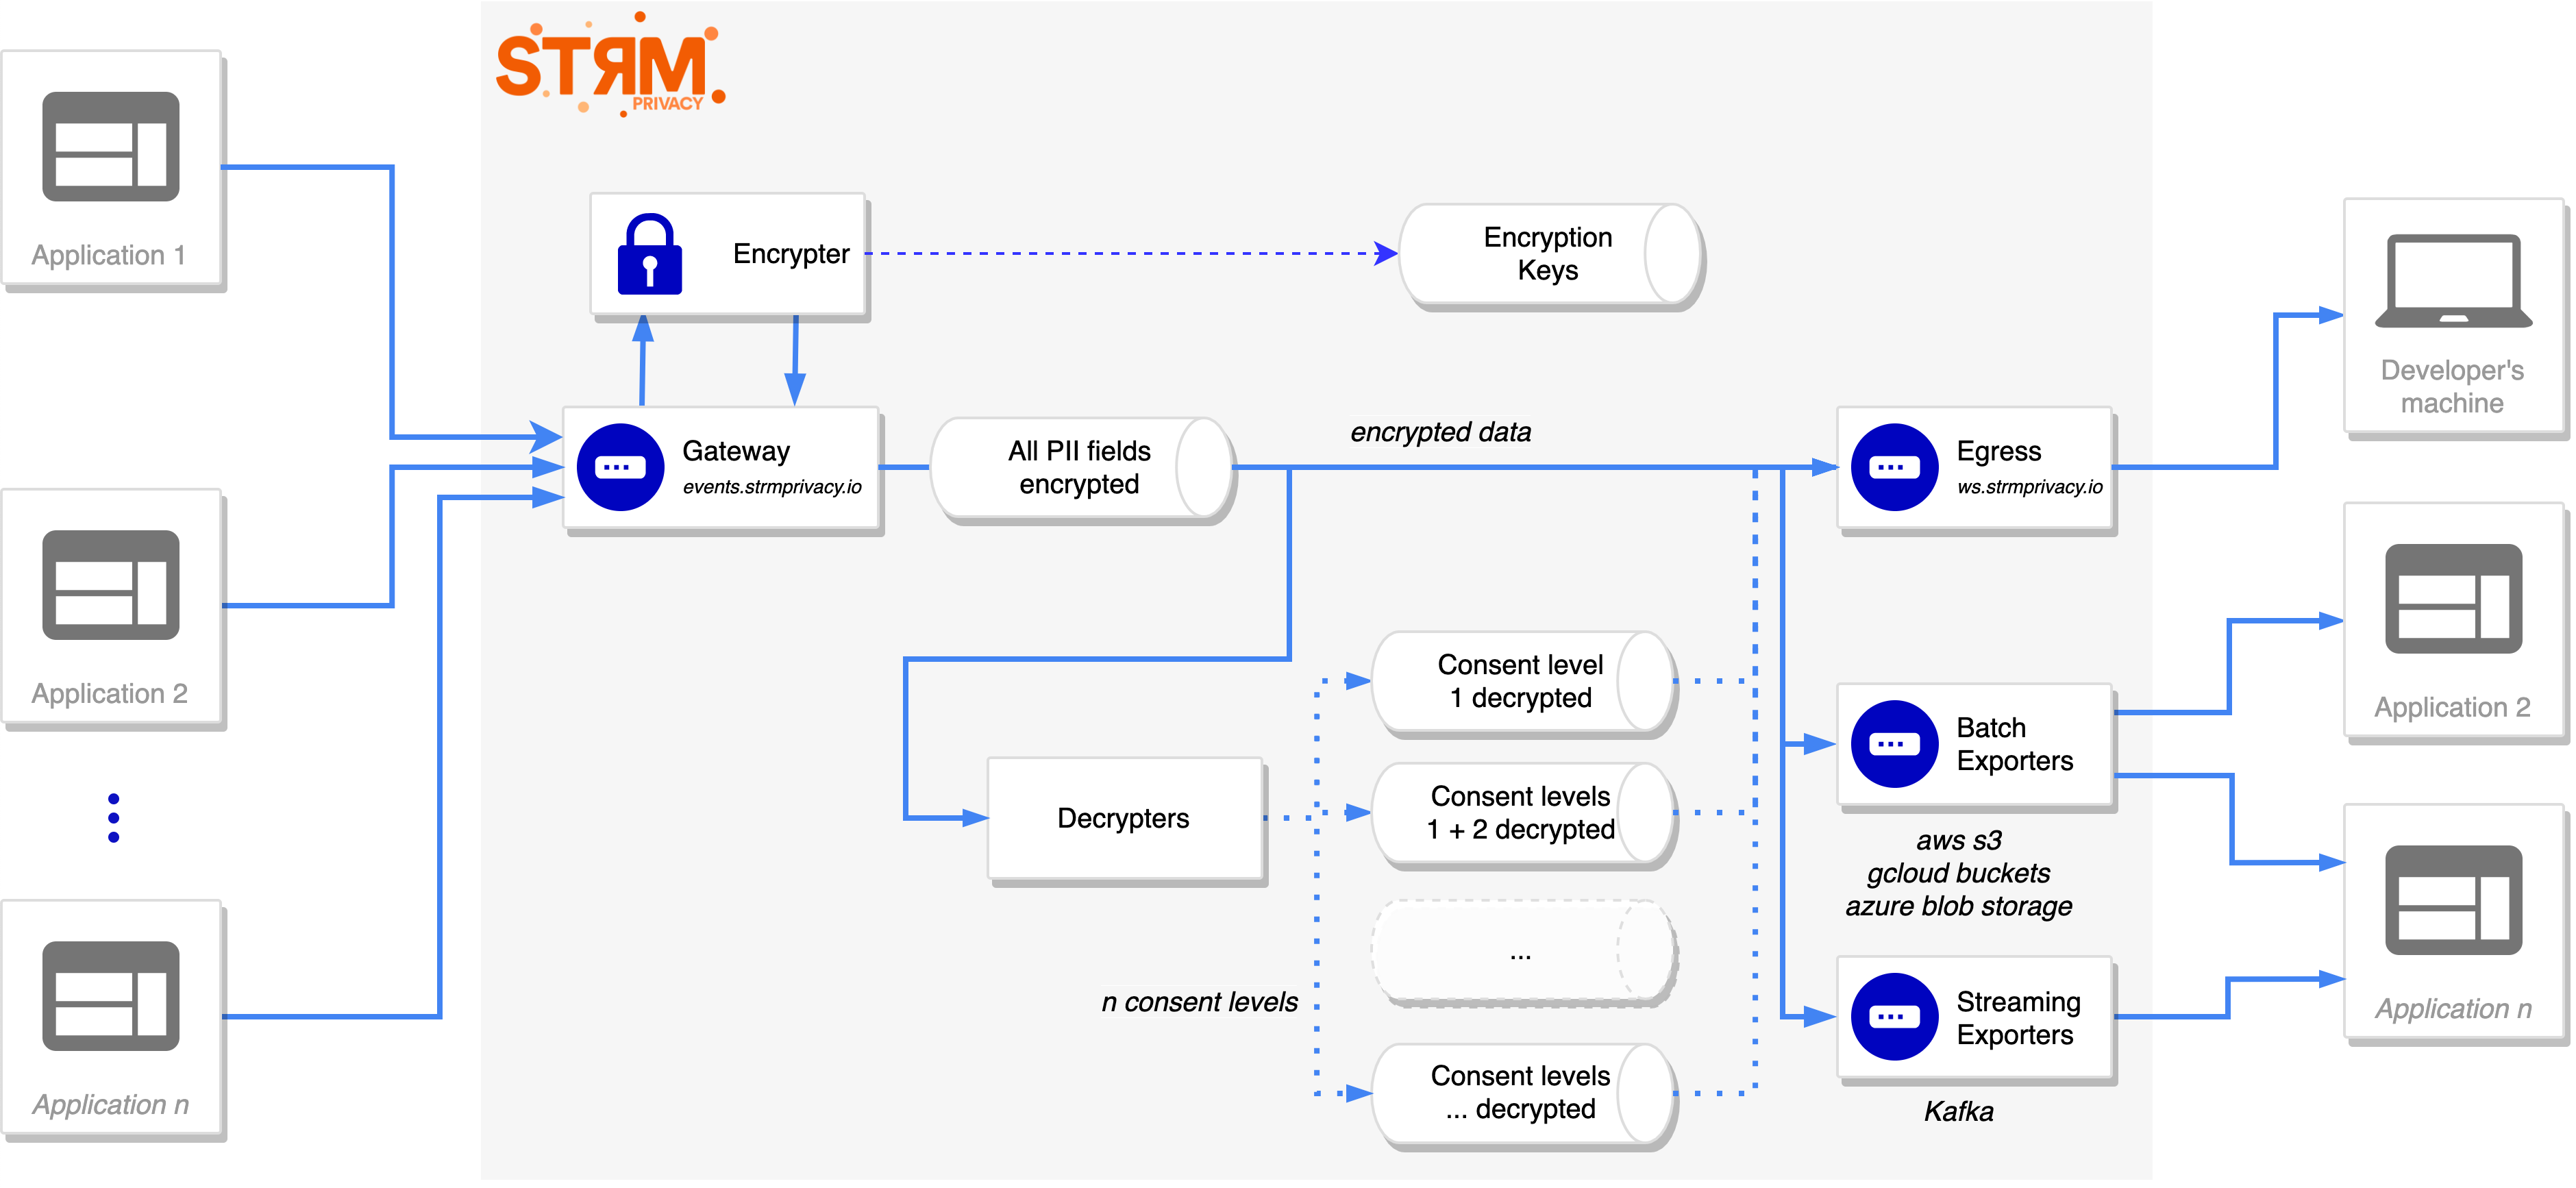
\includegraphics[width=\linewidth]{figs/arch.png}}
  \caption{\label{fig:arch}STRM Privacy High Level Architecture}
\end{figure}

We apply encryption methods beyond just obfuscating underlying field values. Through key rotations on links inside the data items, privacy transformations such as masking or anonymization can be performed in real-time. Combined with the purpose and consent binding, we can split the incoming data and create purpose-driven data interfaces that downstream applications or teams can consume without privacy concerns. 

The encryption mechanism will assign the same encryption key to the same value of a specific data item field. As the same value for a field in the data item yields the same cipher-text value, the integrity between events is retained. With a time-based encryption key rotation (i.e. the privacy algorithm) we can consider the resulting encrypted data stream to be \emph{not privacy sensitive anymore}. Next to that, in case a data owner requests to \textit{be forgotten}, throwing away the encryption key destroys all personality dimensions inside the data, but helps to retain the utility of the non-sensitive fields. This process is also known as crypto-shredding \cite{comptonassured}.

In sum, our architecture allows to encode privacy into a data point from the moment of collection onward, enforcing that personal data is only available when the purpose allows it, while retaining important utility of the data. Our documentation \cite{strmprivacydocs} provides a deep dive into all the various components that drive this architecture.

\section{Related Work}
At this point, we positioned the need and guiding principles for building real-world data systems from privacy forward. We have described how the architecture of STRM Privacy follows these principles through an \textit{event-based} component, a \textit{privacy} component, and a \textit{data quality} component. 

Evidently, specific technologies exist for the various components such an architecture requires. First, for data processing in streaming fashion, there are various established technologies, such as Apache Kafka, Kafka Streams, Apache Beam, and many other Open Source and commercial solutions (see e.g. \cite{isah2019survey} or \cite{mehmood2020challenges}).

Secondly, we emphasize that specific solutions in the realm of Privacy Enhancing Technologies are on the rise that warrant privacy through different approaches (see for an overview \cite{Polonetsky2021review}). Their goal generally is to destroy identification in data, while maintaining the same (statistical) characteristics to sufficiently represent the original data to conduct operations (see for example earlier IEEE publications \cite{li2007t} or \cite{zhou2008brief}). For example, solutions include Synthetic Data Generation, obfuscating data on existing data sets, and data encryption at rest. Some challenges remain, e.g. with obfuscation, one should ensure that the obfuscated data is not susceptible to linkage attacks combining obfuscated data with other data to de-anonymize the data \cite{merener2012theoretical}. An important limitation of these approaches is that they are currently not able to accommodate real-time transformations and embedding in operational data systems \cite{anderson2014synthetic}, and often require existing data sets that might be collected in violation. 

Finally, \textit{data quality} is considered to be of pivotal importance for any downstream application \cite{cai2015challenges},\cite{breck2019data}. Hence, both traditional ETL tooling and novel ML supported techniques (see for example \cite{grafberger2021lightweight}) enable both validating and enriching data at ingest or even in transit. Metadata management is an important adjacent field, which could further enrich \textit{data usability} in data pipelines \cite{sawadogo2021data}, although scalability of such systems is still challenging \cite{singh2018scalable}. 

\section{Conclusion}
In this paper we argued that building data systems for privacy in real-world production settings should be guided by a core set of principles derived from legislative and \textit{Privacy by Design} frameworks. This enables closing an existing gap between the policy perspective of privacy and the operational reality of data systems.

Existing \textit{Privacy Enhancing Technologies} focus mostly on heavy computational tasks, such as synthetics, at the cost of latency and compute power. They are generally best suited to existing data sets, not in-flight data. Critically, data teams should not treat privacy as an access problem and shift their data privacy efforts to the point of data collection (i.e. "shift left") to better position for compliance. When employing data contracts to encode privacy and tight coupling to privacy transformations, scalable data systems that retain performance and data quality are achievable. They can be compatible with progressive data system philosophies (i.e. the Modern Data Stack or Data Mesh \cite{machado2022data}). In effect, this lowers the \textit{Cost of Privacy} through better data usability, reduced compliance risks and improved coordination between engineering teams and legal departments.

To the best of our knowledge, no other solution exists that focuses on encoding privacy inside data, combined with proven technologies for streaming infrastructure to minimize impact in latency and performance to complement existing data systems. Apart from a better modus operandi for data systems in general, such systems can drive valuable innovation like real-time machine learning while respecting end-user privacy (and thus privacy regulations), and bring privacy by design for data to a much wider audience. We happily invite the community to further extend the collective body of knowledge, by providing feedback or iterations to our work.

% \bibliographystyle{plain}
% \bibliography{bibliography}

\begin{thebibliography}{10}
\itemsep=1pt
\begin{small}

\bibitem{abiteboul2019transparency}
Serge Abiteboul and Julia Stoyanovich.
\newblock Transparency, fairness, data protection, neutrality: Data management
  challenges in the face of new regulation.
\newblock {\em Journal of Data and Information Quality (JDIQ)}, 11(3):1--9,
  2019.

\bibitem{akamai}
Akamai.
\newblock {Akamai Online Retail Performance Report}.
\newblock
  \url{https://www.akamai.com/newsroom/press-release/akamai-releases-spring-2017-state-of-online-retail-performance-report},
  2017.

\bibitem{anderson2014synthetic}
Jason~W Anderson, Ken~E Kennedy, Linh~B Ngo, Andre Luckow, and Amy~W Apon.
\newblock Synthetic data generation for the internet of things.
\newblock In {\em 2014 IEEE International Conference on Big Data (Big Data)},
  pages 171--176. IEEE, 2014.

\bibitem{barhamgi2022special}
Mahmoud Barhamgi and Elisa Bertino.
\newblock Special issue on data transparency—data quality, annotation, and
  provenance.
\newblock {\em Journal of Data and Information Quality (JDIQ)}, 14(1):1--3,
  2022.

\bibitem{bhajaria2022data}
N.~Bhajaria.
\newblock {\em Data Privacy: A Runbook for Engineers}.
\newblock Manning, 2022.

\bibitem{breck2019data}
Eric Breck, Neoklis Polyzotis, Sudip Roy, Steven Whang, and Martin Zinkevich.
\newblock Data validation for machine learning.
\newblock In {\em MLSys}, 2019.

\bibitem{bridge2018}
Mind~the Bridge.
\newblock Gdpr and beyond recommendations from a transatlantic perspective, Dec
  2018.

\bibitem{cai2015challenges}
Li~Cai and Yangyong Zhu.
\newblock The challenges of data quality and data quality assessment in the big
  data era.
\newblock {\em Data science journal}, 14, 2015.

\bibitem{cavoukian1997}
Ann Cavoukian.
\newblock Privacy by design: The 7 foundational principles, 1997.

\bibitem{cichy2019overview}
Corinna Cichy and Stefan Rass.
\newblock An overview of data quality frameworks.
\newblock {\em IEEE Access}, 7:24634--24648, 2019.

\bibitem{comptonassured}
Andrea Compton.
\newblock Assured deletion in the cloud.
\newblock
  \url{https://www.cs.tufts.edu/comp/116/archive/fall2014/acompton.pdf}.

\bibitem{fu2015streaming}
Maosong Fu, Sailesh Mittal, Vikas Kedigehalli, Karthik Ramasamy, Michael Barry,
  Andrew Jorgensen, Christopher Kellogg, Neng Lu, Bill Graham, and Jingwei Wu.
\newblock Streaming@ twitter.
\newblock {\em IEEE Data Eng. Bull.}, 38(4):15--27, 2015.

\bibitem{grafberger2021lightweight}
Stefan Grafberger, Julia Stoyanovich, and Sebastian Schelter.
\newblock Lightweight inspection of data preprocessing in native machine
  learning pipelines.
\newblock In {\em Conference on Innovative Data Systems Research (CIDR)}, 2021.

\bibitem{iapp2017}
Looking to comply with gdpr? here's a primer on anonymization and pseudonymization.
\newblock
  \url{https://iapp.org/news/a/looking-to-comply-with-gdpr-heres-a-primer-on-anonymization-and-pseudonymization/}.

\bibitem{isah2019survey}
Haruna Isah, Tariq Abughofa, Sazia Mahfuz, Dharmitha Ajerla, Farhana
  Zulkernine, and Shahzad Khan.
\newblock A survey of distributed data stream processing frameworks.
\newblock {\em IEEE Access}, 7:154300--154316, 2019.

\bibitem{korenhof2015timing}
Paulan Korenhof, Jef Ausloos, Ivan Szekely, Meg Ambrose, Giovanni Sartor, and
  Ronald Leenes.
\newblock Timing the right to be forgotten: A study into “time” as a factor
  in deciding about retention or erasure of data.
\newblock In {\em Reforming European data protection law}, pages 171--201.
  Springer, 2015.

\bibitem{li2007t}
Ninghui Li, Tiancheng Li, and Suresh Venkatasubramanian.
\newblock t-closeness: Privacy beyond k-anonymity and l-diversity.
\newblock In {\em 2007 IEEE 23rd international conference on data engineering},
  pages 106--115. IEEE, 2007.

\bibitem{machado2022data}
In{\^e}s~Ara{\'u}jo Machado, Carlos Costa, and Maribel~Yasmina Santos.
\newblock Data mesh: Concepts and principles of a paradigm shift in data
  architectures.
\newblock {\em Procedia Computer Science}, 196:263--271, 2022.

\bibitem{mehmood2020challenges}
Erum Mehmood and Tayyaba Anees.
\newblock Challenges and solutions for processing real-time big data stream: A
  systematic literature review.
\newblock {\em IEEE Access}, 8:119123--119143, 2020.

\bibitem{merener2012theoretical}
Martin~M Merener.
\newblock Theoretical results on de-anonymization via linkage attacks.
\newblock {\em Trans. Data Priv.}, 5(2):377--402, 2012.

\bibitem{Polonetsky2021review}
Jules Polonetsky and Tim Sparapani.
\newblock A review of the privacy-enhancing technologies software market.
\newblock {\em IEEE Security Privacy}, 19(6):119--122, 2021.

\bibitem{sawadogo2021data}
Pegdwend{\'e} Sawadogo and J{\'e}r{\^o}me Darmont.
\newblock On data lake architectures and metadata management.
\newblock {\em Journal of Intelligent Information Systems}, 56(1):97--120,
  2021.

\bibitem{singh2018scalable}
Harcharan~Jit Singh and Seema Bawa.
\newblock Scalable metadata management techniques for ultra-large distributed
  storage systems--a systematic review.
\newblock {\em ACM Computing Surveys (CSUR)}, 51(4):1--37, 2018.

\bibitem{soria2016big}
Jordi Soria-Comas and Josep Domingo-Ferrer.
\newblock Big data privacy: challenges to privacy principles and models.
\newblock {\em Data Science and Engineering}, 1(1):21--28, 2016.

\bibitem{strmprivacydocs}
{STRM Privacy documentation}.
\newblock \url{https://docs.strmprivacy.io/}.

\bibitem{GDPR}
European Union.
\newblock {General Data Protection Regulation}.
\newblock
  \url{https://eur-lex.europa.eu/legal-content/EN/TXT/HTML/?uri=CELEX:32016R0679&from=EN},
  2016.

\bibitem{eugeneyan2021}
Eugene Yan.
\newblock Real-time machine learning for recommendations.
\newblock \url{https://eugeneyan.com/writing/real-time-recommendations/}, 2021.
\newblock Post published on 10 Jan 2021.

\bibitem{zhou2008brief}
Bin Zhou, Jian Pei, and WoShun Luk.
\newblock A brief survey on anonymization techniques for privacy preserving
  publishing of social network data.
\newblock {\em ACM Sigkdd Explorations Newsletter}, 10(2):12--22, 2008.


\end{small}
\end{thebibliography}

\end{document}